\subsubsection{Definição do instrumento e do tempo}\label{sec:define_instr}

Seu início é um pequeno comentário que contêm o nome do executante e seu email para contato (primeiros sete segundos), bem como a escrita de um código que inicializa o NI-Akoustik (até 0$'$43$''$, ver \autoref{fig:SIK_piano}). 

%%%%%%%%%%%%%%%%%%%%%%%%%%%%%%%%%%%%%%%%%
\begin{example}{Definição de instrumento}
  \centering 
Primeiros eventos musicais gerados a partir das primeiras estruturas válidas de código. \textbf{Fonte}: \cite{sorensen_youtube_2014}.
  \begin{minted}[fontsize=\footnotesize]{cl}
    ;;;;;;;;;;;;;;;;;;;;;;;;;;;;;;;;;;;;;;;;;;;;;;;;;
    ;; Andrew Sorensen andrew@moso.com.au
    (define piano (au:make-node "aumu" "NaDd" "-NI-"))
    (au:connect-node piano 0 *au:output-node* 0)
    (au:update-graph)

    (au:load-preset piano "/tmp/convert_grand.aupreset")
  \end{minted}
  \label{fig:SIK_piano}
\end{example}
%%%%%%%%%%%%%%%%%%%%%%%%%%%%%%%%%%%%%%%%%

\newcommand{\tempo}[2]{#1$'$#2$''$}

Em \tempo{0}{52} Sorensen define um tempo base (ver \autoref{fig:SIK_metro}). Em seguida, Sorensen apaga o código para então iniciar definições de notas (\tempo{0}{54}).

%%%%%%%%%%%%%%%%%%%%%%%%%%%%%%%%%%%%%%%%%
\begin{example}{Definição de tempo}
  \centering
  Definição do tempo base. \textbf{Fonte}: \cite{sorensen_youtube_2014}.
  \begin{minted}[fontsize=\footnotesize]{cl}
    (define *metro* (make-metro 110))
  \end{minted}
  \label{fig:SIK_metro}
\end{example}
%%%%%%%%%%%%%%%%%%%%%%%%%%%%%%%%%%%%%%%%%

\subsubsection{Definição de uma sequência de blocos}

Até \tempo{1}{07}, uma função auxiliar é definida como um laço iterativo (\mint{cl}|pc:cb-for-each-p|) chama por acordes (\mint{cl}|chords|), cujos parâmetros são três: i) \mint{cl}|piano (pc:make-chord 50 70 2 (pc:diatonic 0 '- degree))|; ii). (ainda não sabemos quais são, o que caracteriza uma memória particular já interiorizada por Sorensen; isto é, ele ensaiou essa improvisação). (que  \ver{fig:SIK_acorde}.  Para cada acorde, é chamada uma a função que ainda não existe, \emph{chords}. Esta função é acompanhada de uma lista de 4 parâmetros (50, 70, 2), e o último,  é uma função  executada

%%%%%%%%%%%%%%%%%%%%%%%%%%%%%%%%%%%%%%%%%
\begin{example}{Definição da sequência de blocos}\label{fig:SIK_acorde}

Criação da rotina que irá executar acordes \cite{sorensen_youtube_2014}.

  \begin{minted}[fontsize=\footnotesize]{cl}
    (pc:cb-for-each-p chords piano
                      (pc:make-chord 50 70 2 (pc:diatonic 0 '- degree))
                      dur)
  \end{minted}
\end{example}
%%%%%%%%%%%%%%%%%%%%%%%%%%%%%%%%%%%%%%%%%

\subsubsection*{Definição de blocos}\label{sec:define_chords}

Em \tempo{1}{08}, a função \emph{chords}, e o o código que executa, surge no fluxo audiovisual, sem nenhum processo de escrita. Este comportamento caracteriza a utilização de, ou uma cópia/cola de texto, ou de uma execução de um macro do editor de texto usado. Macros são pequenos programas no editor que auxiliam o processo de produção do código. De qualquer forma é importante salientar que o código é preparado \cite{sorensen_youtube_2014}.

%%%%%%%%%%%%%%%%%%%%%%%%%%%%%%%%%%%%%%%%%%%%%%%%
\begin{example}{Algoritmo que define os acordes}

O algoritmo apresenta apenas uma propriedade, tempo (\verb|time|).

\begin{minted}[fontsize=\footnotesize]{cl}
    (define chords
       (lambda (time)
          (for-each (lambda (p)
                       (play-note (*metro* time) piano p 80 (*metro* 'dur dur)))                                 
                    (pc:make-chord 50 70 2 (pc:diatonic 0 (quote -) degree)))
          (callback (*metro* (+ time (* .5 dur))) chords (+ time dur))))
    
     (chords (*metro* 'get-beat 4.0) 'i 3.0)
\end{minted}

Para cada momento definido por \verb|time|,

\begin{minted}[fontsize=\footnotesize]{cl}
(define chords
   (lambda (time) ... ))
\end{minted}

É executado um laço iterativo, \verb|for-each|, 

\begin{minted}[fontsize=\footnotesize]{cl}
(for-each (lambda (p)
             (play-note (*metro* time) piano p 80 (*metro* 'dur dur)))                                 
          (pc:make-chord 50 70 2 (pc:diatonic 0 (quote -) degree)))
\end{minted}

que cria uma nota, com uma altura \verb|p|, 

\begin{minted}[fontsize=\footnotesize]{cl}
(play-note (*metro* time) piano p 80 (*metro* 'dur dur))
\end{minted}

para cada díade definida em \verb|pc:make-chord|

\begin{minted}[fontsize=\footnotesize]{cl}
(pc:make-chord 50 70 2 (pc:diatonic 0 (quote -) degree)))
\end{minted}

\verb|play-note| é definido com os seguintes argumentos, momento de execução ($time~\Rightarrow~(*metro* time)$), o instrumento tocado, ($instr~\Rightarrow~piano$), a altura ($pitch~\Rightarrow~p$), o volume ($vol~\Rightarrow~80$) e a duração do acorde ($dur~\Rightarrow~(*metro* 'dur dur)$)\disponivelem{https://github.com/digego/extempore/blob/5aec8b35c6b3058d1c66de7abf752dc667ab61e4/libs/core/instruments-scm.xtm}. A criação da díada, através de \verb|pc:make-chord|, é realizada no âmbito de um Ré 2 (MIDI 50) e Si bemol 3 (MIDI 70). O resultado não é previsível, e depende de regras de qualidade, que apresentaremos adiante, para classificar os \emph{pitch class} dentro de um grau de um campo harmônico:

A abreviação \verb|pc| significa \emph{pitch class}, e a função \verb|pc:make-chord| significa que a função cria um acorde segundo parâmetros definidos no código-fonte do \emph{Extempore} \disponivelem{https://github.com/digego/extempore/blob/master/libs/core/pc_ivl.xtm}:

\begin{citacao}
\traducao{Cria uma lista do ``número'' $[$com$]$ alturas entre limites ``menor'' e ``maior'' do \emph{pc} dado. Uma divisão dos limites, pelo número de elementos requisitados, decompõem a seleção em extensões diferentes, do qual cada altura é selecionada. \emph{make-chord} tenta selecionar alturas para todos os graus do \emph{pc}. É possível, para  os elementos de um acorde resultarem em -1, se não existir nenhum \emph{pc} para a extensão dada. $[$É$]$ não-determinístico (i.e., resultados variam com o tempo). Argumento 1: limite menor (inclusivo). Argumento 2: Limite maior (exclusivo). Argumento 3: Número de alturas no acorde. Argumento 4: \emph{pitch class} \cite{swift_playingII_2012}.}{Creates a list of "number" pitches between "lower" and "upper" bounds from the given "pc". A division of the bounds by the number of elements requested breaks down the selection into equal ranges from which each pitch is selected.  \emph{make-chord} attempts to select pitches of all degrees of the pc.  It is possible for elements of the returned chord to be -1 if no possible pc is available for the given range. Non-deterministic (i.e. result can vary each time). arg1: lower bound (inclusive).  arg2: upper bound (exclusive). arg3: number of pitches in chord.  arg4: pitch class}
\end{citacao}

No código abaixo, \verb|callback| é executado após a criação do acorde, e ele mesmo executa outros acordes, com base no tempo do que já foi executado:

\begin{minted}[fontsize=\footnotesize]{cl}
(callback (*metro* (+ time (* .5 dur))) chords (+ time dur))))
\end{minted}
\end{example}
%%%%%%%%%%%%%%%%%%%%%%%%%%%%%%%%%%%%%%%%%%%%%%%%


Este código inicial é então modificado, e finalizado em \tempo{1}{57}, momento em que aparece uma figura, duas díades, um intervalo de quarta justa entre Sol 2 (MIDI 55) e Dó 3 (MIDI 60). entre Mi bemol 2 (MIDI 51) e Dó 3 (MIDI 60).

%%%%%%%%%%%%%%%%%%%%%%%%%%%%%%%%%%%%%%%%%%%%%%%%
\begin{example}{Estratégia transversal}
\begin{minted}[fontsize=\footnotesize]{cl}
    (define chords
       (lambda (time degree dur)
          (if (member degree '(i)) (set! dur 3.0))
          (for-each (lambda (p)
                       (play-note (*metro* time) piano p
                                  (+ 50 (* 20 (cos (* pi time))))
                                  (*metro* 'dur dur)))
                    (pc:make-chord 50 70 2 (pc:diatonic 0 (quote -) degree)))
          (callback (*metro*) (+ time (* .5 dur))) chords (+ time dur)
                    (random (assoc degree '((i vii)
                                            (vii i))))
                    dur))
    
     (chords (*metro* 'get-beat 4.0) 'i 3.0)
\end{minted}
\end{example}
%%%%%%%%%%%%%%%%%%%%%%%%%%%%%%%%%%%%%%%%%%%%%%%%

Duas transcrições seguem uma estrutura literal do código, e uma perceptiva \ver{fig:ask2}, sendo que escolhemos seguir com a segunda, por simbolizar pequenos figuras musicais, como neumas \ver{fig:bipunctum}. Na mão direita, um \emph{bipunctum} , e na mão esquerda, uma \emph{clivis} \ver{fig:bipunctum}. 

\begin{figure}[!h]
  \centering
  \input{./ask1}
  \input{./ask2}
  \caption{Transcrição literal e perceptiva do primeiro evento em \emph{A Study in Keith}. \textbf{Fonte}: autor.}
  \label{fig:ask1}
\end{figure}


\begin{figure}[!h]
  \centering
  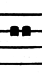
\includegraphics[scale=1]{imagens/bipunctum.png}
  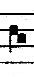
\includegraphics[scale=1]{imagens/clivis.png}
  \caption{Notação neumática para um bipunctum, e uma \emph{clivis}, no primeiro evento sonoro. Fonte: wikimedia.org.}
  \label{fig:bipunctum}
\end{figure}

 É importante notar que algumas alterações são feitas. A primeira delas é definir outros argumentos para \verb|chords|, como um acorde localizado em um grau de um campo harmônico abstrato, e a duração do acorde executado:

%%%%%%%%%%%%%%%%%%%%%%%%%%%%%%%%%%%%%%%%%%%%%%%%
\begin{example}{Modificação do código original}
\begin{minted}[fontsize=\footnotesize]{cl}
    (define chords
       (lambda (time degree dur) ...))
\end{minted}
%%%%%%%%%%%%%%%%%%%%%%%%%%%%%%%%%%%%%%%%%%%%%%%%

A segunda delas é a indicação de uma situação condicional: se o grau a ser executado for a tônica menor, configure a duração deste acorde para três unidades de tempo,

\begin{minted}[fontsize=\footnotesize]{cl}
(define chords
   (lambda (time degree dur)
      (if (member degree '(i)) (set! dur 3.0)) ... ))
\end{minted}

A terceira modifica o volume das notas:

\begin{minted}[fontsize=\footnotesize]{cl}
(play-note (*metro* time) piano p
           (+ 50 (* 20 (cos (* pi time))))
           (*metro* 'dur dur))
\end{minted}

Onde a a dinâmica notada, no exemplo anterior, ocorre como um comportamento periódico de volumes máximos (fortes), e mínimos (pianos), em, proporcional ao cosseno do tempo instantâneo. 

\begin{minted}[fontsize=\footnotesize]{cl}
(+ 50 (* 20 (cos (* pi time))))
\end{minted}
\end{example}

A estrutura interna da estratégia \verb|chords| explicita algumas regras de qualidade, bem como permite apresentar uma primieira sequência de blocos de eventos \pressingthree{K}{ask}{0}, um conjunto de características \pressingthree{F}{ask}{0} e um pequeno grupo de objetos \pressingthree{O}{ask}{0}. Um conjunto de características é definido pelo momento de execução do evento,\pressingthree{F}{ask}{0}, o grau, \pressingthree{F}{ask}{1}, e a duração deste evento, \pressingthree{F}{ask}{2}. É importante destacar que o momento de execução é relativo ao tempo base, definido dentro do padrão \verb|* metro *| (que será explicado a seguir) de um campo harmônico, onde i representa uma tônica menor, e vii, um acorde de sétimo grau, e a duração deste acorde

\begin{example}{Regra de qualidade \csf{R}{ask}.}
\begin{minted}[fontsize=\scriptsize]{cl}
( ... (... (callback (*metro*) (+ time (* .5 dur))) chords (+ time dur)
                    (random (assoc degree '((i vii)
                                            (vii i))))
                    dur))
\end{minted}

Cujas características irão gerar blocos de eventos, e sequências de blocos de eventos:

\begin{minted}[fontsize=\scriptsize]{cl}
( ...
  (lambda (time degree dur) ... ))
\end{minted}

O que permite executar como:
\begin{minted}[fontsize=\scriptsize]{cl}
(chords (*metro* 'get-beat 4.0) 'i 3.0)
\end{minted}
\end{example}




\subsection{Segundo Evento Sonoro}\label{sec:segundoevento}

Uma escuta investigativa desta performance considerou o resultado sonoro gerador como replicante de uma escrita contrapontística modal, não-estrita, inicialmente à duas vozes em primeira espécie, que lembra um canto religioso.

Sorensen define um tempo regular de 110 BPM durante o momento de silêncio Os primeiros eventos sonoros que ocorrem após o momento de silêncio foram transcritos considerando a percepção dos tempos fortes e fracos. Isto é, enquanto Sorensen define um tempo regular de 110 BPM, o processo de transcrição
de maneira aproximada em um tempo regular de aproximadamente 40 BPM. A partir disso, cada compasso desta transcrição são dois compassos do vídeo. Segundo o próprio vídeo, o tempo é definido por 110 BPM e cada nota inicial é de quatro tempos, mas que irá sofrer alterações. 

A \autoref{fig:SIK_acorde2} indica que um jogo entre primeiro grau menor, e sétimo grau diminuto será conduzido  (ver \autoref{fig:SIKinicio}).

\begin{figure}[!h]
  \centering
  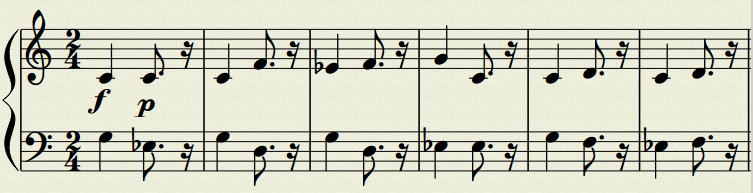
\includegraphics[scale=0.5]{imagens/SIK_motivo.png}
  \caption{Primeiros eventos musicais gerados a partir das primeiras estruturas válidas de código. \textbf{Fonte}: autor.}
  \label{fig:SIKinicio}
\end{figure}

Uma pequena transcrição de uma primeira seção da improvisação é apresentada na \autoref{app:studyinkeith}: uma primeira seção da peça, que vai do 1$'$53$''$ até 4$'$55$''$, pode ser descrita como: um contraponto, inicialmente à duas vozes em primeira espécie (dó eólio), que sofre perturbações sistêmicas. Tais perturbações parecem ser derivadas das intervenções de Sorensen no código do programa.

Tais perturbações criam variações na acentuação, bem como adicionam novas figuras de ritmo, de maneira bastante gradual (ver \autoref{fig:perturba}).

\begin{figure}[!h]
  \centering
  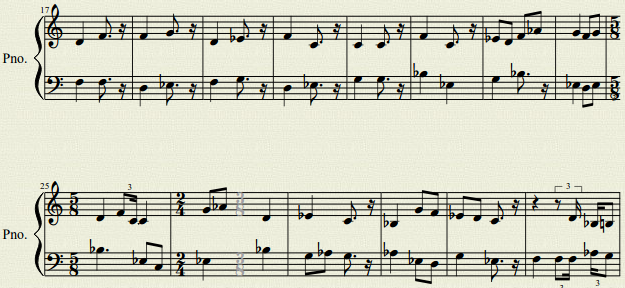
\includegraphics[scale=0.5]{imagens/SIK_perturba.png}
  \caption{Primeiros perturbações sistêmicas. \textbf{Fonte}: autor.}
  \label{fig:SIKinicio}
\end{figure}

No ponto culminante da peça podemos escutar um contraponto florido, adicionado de um ostinato com uma única nota, e algumas intervenções de gestos, arpejos ou escalas em alta velocidade.\todo{\tiny Este conceito nos pareceu bastante similar àquele apresentado por \citeonline{hiller_experimental_1959}. HillerDurante um breve período, algumas regras de contraponto não mantidas}


\subsection{Terceiro Evento Sonoro}\label{sec:terceiro evento}